% 原文PDF206の6.5見出しからPDF227末まで。
\subsectionlink{Chan--Paton因子とゲージ相互作用}\label{sec:6.5}

本節では、開弦の質量のないベクトル状態の相互作用を考える。議論を少し興味深いものにするため、まず開弦理論の一般化を導入する。

第3章末では、非常に広いクラスのボソン弦理論を導入したが、相互作用を初めて調べるここでは、最も単純な平坦な26次元の場合に注目する。これは対称性の観点から考えられる。この理論は最大の26次元 Poincaré 不変性をもつ。閉ボソン弦では、この対称性をもつ理論はこれだけである。証明の概略は次のとおりである。時空の並進に対する世界面の Noether カレントは、ウェイト $(1,0)$ と $(0,1)$ の成分をもつ。第2.9節の議論によれば、これらのカレントは $z$ または $\bar z$ に関して正則となる。本章の計算で見たように、これだけで、すべての期待値を決定するのに十分である。

\begin{figure}[tbp]
\centering
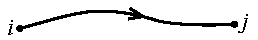
\includegraphics[width=0.52\linewidth]{figures/fig_6_4.pdf}
\caption{Chan--Paton 自由度をもつ開弦。}
\label{fig:6.4}
\end{figure}

しかし開弦理論には一般化がある。開弦は境界、すなわち端点をもつ。特別な点をもつ量子系では、内部を伝播する場に加えて、その点に存在する自由度を設けるのが自然である。開弦の各端に、$n$ 個の状態のいずれかをとりうる、Chan--Paton 自由度と呼ばれる新しい自由度を加えよう。すると弦状態の基底は
\begin{equation}
|N;k;ij\rangle
\tag{6.5.1}\label{eq:6.5.1}
\end{equation}
となる。ここで $i,j$ は左端と右端の状態を表し、1から $n$ までの値をとる。エネルギー運動量テンソルは以前と同じものと定義し、新しい自由度には依存させない。したがって、共形不変性は自動的に成り立つ。Chan--Paton 自由度は不変なので、Poincaré 不変性も自動的に成り立つ。これらの新しい自由度の世界面上の力学は自明だが、時空の物理には大きな影響を及ぼす。

強い相互作用の弦理論では、これを導入する動機は $SU(3)$ のフレーバー量子数を導入することにあった。端点は、カラー電気束管で結ばれたクォークと反クォークのようなものである。ここでは、与えられた対称性をもつすべての可能性を考えるという一般的な枠組みから動機付けている。第8章では Chan--Paton 自由度に新しい解釈を与え、第14章ではさらに解釈を精密化する可能性を述べる。

今や $n^2$ 個のスカラータキオン、$n^2$ 個の質量のないベクトルボソンなどがある。
\begin{equation}
\operatorname{Tr}(\lambda^a\lambda^b)=\delta^{ab}
\tag{6.5.2}\label{eq:6.5.2}
\end{equation}
と規格化した $n^2$ 個の Hermite 行列 $\lambda^a_{ij}$ は、二つの端点の状態の完全系である。これらは $U(n)$ の表現行列なので、質量のないベクトルは $U(n)$ ゲージ対称性に対応すると推測できる。間もなく、実際にそうであることが分かる。

基底を
\begin{equation}
|N;k;a\rangle=\sum_{i,j=1}^{n}|N;k;ij\rangle\lambda^a_{ij}
\tag{6.5.3}\label{eq:6.5.3}
\end{equation}
と定義する。図\hyperref[fig:6.2]{6.2}(a) に示した4タキオン振幅を考えよう。そこでは頂点演算子が巡回順序1234に並んでいる。Chan--Paton 自由度は Hamiltonian に現れないので、その状態は頂点演算子の間で時間発展しない。タキオン1の右端は、タキオン2の左端と同じ状態でなければならず、以下も同様である。したがって、図6.2(a)の振幅には、各タキオンの Chan--Paton 波動関数の重なりから、付加的な因子
\begin{equation}
\operatorname{Tr}(\lambda^{a_1}\lambda^{a_2}\lambda^{a_3}\lambda^{a_4})
\tag{6.5.4}\label{eq:6.5.4}
\end{equation}
が含まれる。この規則は任意の振幅に一般化される。各頂点演算子は端点自由度の波動関数から来る Chan--Paton 因子 $\lambda^a_{ij}$ を含み、各世界面の振幅には、それぞれの境界に沿って並べた Chan--Paton 因子のトレースが掛けられる。

3タキオン振幅は
\begin{equation}
\begin{aligned}
S_{D_2}(k_1,a_1;k_2,a_2;k_3,a_3)
={}&\frac{ig_{\mathrm o}}{\alpha'}(2\pi)^{26}
\delta^{26}\left(\sum_i k_i\right)\\
&\times\operatorname{Tr}
(\lambda^{a_1}\lambda^{a_2}\lambda^{a_3}
+\lambda^{a_1}\lambda^{a_3}\lambda^{a_2})
\end{aligned}
\tag{6.5.5}\label{eq:6.5.5}
\end{equation}
となり、今度は二つの巡回順序に異なる Chan--Paton トレースが伴う。4タキオン振幅は
\begin{equation}
\begin{aligned}
&S_{D_2}(k_1,a_1;k_2,a_2;k_3,a_3;k_4,a_4)
=\frac{ig_{\mathrm o}^2}{\alpha'}(2\pi)^{26}
\delta^{26}\left(\sum_i k_i\right)\\
&\quad\times\Bigl[
\operatorname{Tr}(\lambda^{a_1}\lambda^{a_2}\lambda^{a_4}\lambda^{a_3}
+\lambda^{a_1}\lambda^{a_3}\lambda^{a_4}\lambda^{a_2})
B(-\alpha_{\mathrm o}(s),-\alpha_{\mathrm o}(t))\\
&\qquad+
\operatorname{Tr}(\lambda^{a_1}\lambda^{a_3}\lambda^{a_2}\lambda^{a_4}
+\lambda^{a_1}\lambda^{a_4}\lambda^{a_2}\lambda^{a_3})
B(-\alpha_{\mathrm o}(t),-\alpha_{\mathrm o}(u))\\
&\qquad+
\operatorname{Tr}(\lambda^{a_1}\lambda^{a_2}\lambda^{a_3}\lambda^{a_4}
+\lambda^{a_1}\lambda^{a_4}\lambda^{a_3}\lambda^{a_2})
B(-\alpha_{\mathrm o}(s),-\alpha_{\mathrm o}(u))
\Bigr].
\end{aligned}
\tag{6.5.6}\label{eq:6.5.6}
\end{equation}
再びユニタリー性の関係\eqref{eq:6.4.13}を考えると、$s=-1/\alpha'$ の極には、左辺で因子
\begin{equation}
\frac14\operatorname{Tr}
\bigl(\{\lambda^{a_1},\lambda^{a_2}\}\{\lambda^{a_3},\lambda^{a_4}\}\bigr)
\tag{6.5.7}\label{eq:6.5.7}
\end{equation}
が、右辺で因子
\begin{equation}
\frac14\sum_a
\operatorname{Tr}\bigl(\{\lambda^{a_1},\lambda^{a_2}\}\lambda^a\bigr)
\operatorname{Tr}\bigl(\{\lambda^{a_3},\lambda^{a_4}\}\lambda^a\bigr)
\tag{6.5.8}\label{eq:6.5.8}
\end{equation}
が付く。この和は中間状態の Chan--Paton 波動関数にわたる。$\lambda^a_{ij}$ の完全性と規格化\eqref{eq:6.5.2}は、任意の行列 $A,B$ に対して
\begin{equation}
\operatorname{Tr}(A\lambda^a)\operatorname{Tr}(B\lambda^a)
=\operatorname{Tr}(AB)
\tag{6.5.9}\label{eq:6.5.9}
\end{equation}
を意味するので、振幅は依然としてユニタリーである。

\subsubsectionlink*{ゲージ相互作用}

ゲージボソン一つとタキオン二つの振幅は
\begin{equation}
\begin{aligned}
&S_{D_2}(k_1,a_1,e_1;k_2,a_2;k_3,a_3)
=-ig'_{\mathrm o}g_{\mathrm o}^2e^{-\lambda}e_{1\mu}\\
&\quad\times
\left\langle
{}^\star_\star c^1\dot X^\mu e^{ik_1\cdot X}(y_1){}^\star_\star
{}^\star_\star c^1 e^{ik_2\cdot X}(y_2){}^\star_\star
{}^\star_\star c^1 e^{ik_3\cdot X}(y_3){}^\star_\star
\right\rangle_{D_2}
\operatorname{Tr}(\lambda^{a_1}\lambda^{a_2}\lambda^{a_3})\\
&\quad+(k_2,a_2)\leftrightarrow(k_3,a_3).
\end{aligned}
\tag{6.5.10}\label{eq:6.5.10}
\end{equation}
ゲージボソンの頂点演算子\eqref{eq:3.6.26}を用いたが、今のところ独立な規格化定数 $g'_{\mathrm o}$ を許している。第6.2節の結果を用いると、$X$ の経路積分は
\begin{equation}
\begin{aligned}
&\left\langle
{}^\star_\star\dot X^\mu e^{ik_1\cdot X}(y_1){}^\star_\star
{}^\star_\star e^{ik_2\cdot X}(y_2){}^\star_\star
{}^\star_\star e^{ik_3\cdot X}(y_3){}^\star_\star
\right\rangle_{D_2}\\
&\quad=-2i\alpha'\left(\frac{k_2^\mu}{y_{12}}+\frac{k_3^\mu}{y_{13}}\right)
iC^X_{D_2}(2\pi)^{26}\delta^{26}\left(\sum_i k_i\right)
|y_{12}|^{2\alpha'k_1\cdot k_2}
|y_{13}|^{2\alpha'k_1\cdot k_3}
|y_{23}|^{2\alpha'k_2\cdot k_3}.
\end{aligned}
\tag{6.5.11}\label{eq:6.5.11}
\end{equation}
運動量保存、質量殻条件、物理的状態条件 $k_1\cdot e_1=0$ を用いると、振幅は
\begin{equation}
\begin{aligned}
&S_{D_2}(k_1,a_1,e_1;k_2,a_2;k_3,a_3)\\
&\quad=-ig'_{\mathrm o}e_1\cdot k_{23}(2\pi)^{26}
\delta^{26}\left(\sum_i k_i\right)
\operatorname{Tr}\bigl(\lambda^{a_1}[\lambda^{a_2},\lambda^{a_3}]\bigr),
\end{aligned}
\tag{6.5.12}\label{eq:6.5.12}
\end{equation}
となる。ここで $k_{ij}\equiv k_i-k_j$ である。これも頂点演算子の位置に依存しない。

4タキオン振幅の $s=0$ の極は、もはや消えない。以前は打ち消し合った項に、今度は異なる順序の Chan--Paton 因子が伴うので、この極は
\begin{equation}
\operatorname{Tr}\bigl([\lambda^{a_1},\lambda^{a_2}]
[\lambda^{a_3},\lambda^{a_4}]\bigr)
\tag{6.5.13}\label{eq:6.5.13}
\end{equation}
に比例する。この極の係数と振幅\eqref{eq:6.5.12}をユニタリー性によって関係付けると、
\begin{equation}
g'_{\mathrm o}=(2\alpha')^{-1/2}g_{\mathrm o}
\tag{6.5.14}\label{eq:6.5.14}
\end{equation}
を得る。これは状態・演算子対応から得られる相対的規格化と同じであり、独立な結合定数は一つしかない。

3ゲージボソン結合についても、同様の計算から
\begin{equation}
\begin{aligned}
&S_{D_2}(k_1,a_1,e_1;k_2,a_2,e_2;k_3,a_3,e_3)\\
&\quad=ig'_{\mathrm o}(2\pi)^{26}\delta^{26}\left(\sum_i k_i\right)
\Bigl(e_1\cdot k_{23}\,e_2\cdot e_3
+e_2\cdot k_{31}\,e_3\cdot e_1
+e_3\cdot k_{12}\,e_1\cdot e_2\\
&\hspace{7em}+\frac{\alpha'}2
e_1\cdot k_{23}\,e_2\cdot k_{31}\,e_3\cdot k_{12}\Bigr)
\operatorname{Tr}\bigl(\lambda^{a_1}[\lambda^{a_2},\lambda^{a_3}]\bigr)
\end{aligned}
\tag{6.5.15}\label{eq:6.5.15}
\end{equation}
が得られる。

運動量の一次まででは、ここまでに得た振幅は時空作用
\begin{equation}
\begin{aligned}
\boldsymbol S=\frac1{g_{\mathrm o}'{}^2}
\int d^{26}x\Bigl[
&-\frac12\operatorname{Tr}(D_\mu\varphi D^\mu\varphi)
+\frac1{2\alpha'}\operatorname{Tr}(\varphi^2)
+\frac{2^{1/2}}{3\alpha'^{1/2}}\operatorname{Tr}(\varphi^3)\\
&-\frac14\operatorname{Tr}(F_{\mu\nu}F^{\mu\nu})
\Bigr]
\end{aligned}
\tag{6.5.16}\label{eq:6.5.16}
\end{equation}
によって再現される。ここでタキオン場 $\varphi$ と Yang--Mills ベクトルポテンシャル $A_\mu$ は、たとえば $A_\mu=A^a_\mu\lambda^a$ のように $n\times n$ 行列で書いている。また、
$D_\mu\varphi=\partial_\mu\varphi-i[A_\mu,\varphi]$、
$F_{\mu\nu}=\partial_\mu A_\nu-\partial_\nu A_\mu-i[A_\mu,A_\nu]$
である。

これは、随伴表現に属するスカラーに結合した $U(n)$ ゲージ場の作用である。Chan--Paton 因子を加えると、必要なゲージ不変の式がちょうど得られた。後でさらに展開するように、弦の摂動論では非物理的状態の分離が保証されるので、ゲージ不変性は自動的に成り立つ。

運動量 $k$ が弦のスケールに比べて小さいとき、開弦の状態は質量のないゲージボソンだけである。第3.7節で述べたように、この極限で物理は質量のない状態の有効場理論に帰着するはずである。したがって、作用\eqref{eq:6.5.16}にタキオンを含めたのは、やや論理的でなかった。説明のためにそうしたが、ここからはゲージボソンに注目しよう。4ゲージボソン振幅は Veneziano 振幅に似た形をしているが、偏極テンソルから来る追加の構造をもつ。これを $\alpha'k^2$ のべきで展開すると、ゼロスロープ極限 $\alpha'\to0$ で残る最初の項は、$s,t,u$ の極の項と定数の和である。整合性により、これは Yang--Mills Lagrangian $F_{\mu\nu}F^{\mu\nu}$ から場の理論で得られる4ゲージボソン振幅に正確に一致することが保証される。ただし、3ゲージボソン振幅\eqref{eq:6.5.15}の $\alpha'k^3$ 次の項に注意しよう。これは Lagrangian に高階微分項
\begin{equation}
-\frac{2i\alpha'}{3g_{\mathrm o}'{}^2}
\operatorname{Tr}(F_\mu{}^\nu F_\nu{}^\omega F_\omega{}^\mu)
\tag{6.5.17}\label{eq:6.5.17}
\end{equation}
があることを意味する。同様に、4点振幅を展開すると、高次の相互作用の無限和が現れる（\eqref{eq:6.5.17}より先の項は、運動学的な理由から3ゲージボソン振幅には寄与しない）。弦のループ振幅も、低エネルギー領域では有効 Lagrangian から得られるループに帰着する。有効作用の通常の論理により、高階微分項は低エネルギーでは重要でなくなる。それらが重要になるスケール $\alpha'k^2\approx1$ は、まさに新しい物理（質量をもつ弦状態）が現れ、有効作用が適用できなくなるところである。

カットオフがあるなら、なぜくりこみ理論が必要なのだろうか。くりこみ理論には依然として内容があり、実際、これこそがその本来の解釈である。すなわち、有効 Lagrangian のパラメーターを除けば、低エネルギーの物理は高エネルギー理論の詳細に依存しない、ということである。これは利点であると同時に欠点でもある。Planck スケールの理論の形を知らなくても、通常の場の量子論を使って加速器エネルギーでの予言ができる一方、粒子加速器の物理によって Planck スケールの理論を探れないことも意味するからである。

弦のスペクトルと振幅には明白な大域的 $U(n)$ 対称性
\begin{equation}
\lambda^a\longrightarrow U\lambda^aU^\dagger
\tag{6.5.18}\label{eq:6.5.18}
\end{equation}
があり、Chan--Paton トレースと状態のノルムを不変に保つ。振幅の詳しい形から、これが実際には時空の局所対称性であることが分かった。世界面の大域的対称性が時空の局所対称性へ昇格するこの現象は、弦理論ではかなり一般的であることが分かるだろう。

開弦のすべての状態は、$U(n)$ 対称性の下で $n\times n$ の随伴表現として変換する。ちなみに、$U(n)$ は単純 Lie 代数ではなく、$U(n)=SU(n)\times U(1)$ である。$U(1)$ ゲージボソン $\lambda_{ij}=\delta_{ij}/n^{1/2}$ は、振幅\eqref{eq:6.5.12}と\eqref{eq:6.5.15}から分離する。$U(1)$ の随伴表現は自明なので、すべての弦状態は $U(1)$ 対称性に関して中性である。

\subsubsectionlink*{向き付けのない弦}

向き付けのない弦への一般化は興味深い。まず Chan--Paton 因子のない理論を考えよう。球面または円板上の $X^\mu$ CFT は Möbius 不変性に加えて、開弦では $\sigma^1\to\pi-\sigma^1$、閉弦では $\sigma^1\to2\pi-\sigma^1$ という向きを反転する対称性の下でも不変である。この世界面のパリティ対称性は演算子 $\Omega$ によって生成される。モード展開から、開弦では
\begin{equation}
\Omega\alpha^\mu_n\Omega^{-1}=(-1)^n\alpha^\mu_n,
\tag{6.5.19}\label{eq:6.5.19}
\end{equation}
閉弦では
\begin{equation}
\Omega\alpha^\mu_n\Omega^{-1}=\widetilde\alpha^\mu_n
\tag{6.5.20}\label{eq:6.5.20}
\end{equation}
が従う。この対称性はゴーストにも拡張されるが、ゴーストはツリーレベルの振幅に固定した因子を与えるだけなので、議論を散漫にしないため、ここでは明示的には扱わない。

タキオンの頂点演算子は、閉弦でも開弦でも世界面パリティの下で偶であり、これによって演算子の符号が決まる（ゴーストを含まない、積分された頂点演算子については明らかであり、固定された演算子も同じように変換しなければならない）。すると、すべての状態をパリティ固有値 $\omega=\pm1$ で分類できる。開弦での関係\eqref{eq:6.5.19}は
\begin{equation}
\Omega|N;k\rangle=\omega_N|N;k\rangle,
\qquad \omega_N=(-1)^{1+\alpha'm^2}
\tag{6.5.21}\label{eq:6.5.21}
\end{equation}
を意味する。世界面パリティは乗法的に保存される。たとえば、3タキオン振幅はゼロでなく、$(+1)^3=1$ と整合する。一方、質量のないベクトルは $\omega=-1$ をもつので、Chan--Paton 自由度がなければ、ベクトル・タキオン・タキオン振幅\eqref{eq:6.5.10}と3ベクトル振幅\eqref{eq:6.5.15}は消えると予想され、実際そのとおりになる（$\lambda^a$ は1に置き換わり、交換子が消える）。世界面パリティによって互いに関係付けられる、異なる巡回順序の寄与が打ち消し合う。

整合的な向き付けのある弦理論が与えられると、スペクトルを $\omega=+1$ の状態に制限することにより、新しい向き付けのない弦理論を作れる。$\alpha'm^2$ が奇数の状態は残り、光子を含む、$\alpha'm^2$ が偶数の状態は存在しなくなる。$\omega$ の保存により、外部状態がすべて $\omega=+1$ ならば、ツリーレベル振幅の中間状態も $\omega=+1$ となることが保証される。したがって、少なくともツリーレベルでは（実際には、第9章で概説するようにすべての次数で）、向き付けのない理論のユニタリー性は、向き付けのある理論のユニタリー性から従う。

向き付けのない理論で主に関心をもつのは、Chan--Paton 因子の扱いである。これらは開弦のそれぞれの端点と同一視したので、世界面パリティは両者を入れ替えなければならない。
\begin{equation}
\Omega|N;k;ij\rangle=\omega_N|N;k;ji\rangle .
\tag{6.5.22}\label{eq:6.5.22}
\end{equation}
これも、向き付けのある理論のすべての振幅の対称性である。向き付けのない理論を作るには、再びスペクトルを世界面パリティ固有値 $\omega=+1$ に制限する。$\lambda^a_{ij}$ の基底を、各行列が対称で $s^a=+1$、または反対称で $s^a=-1$ となるように選ぶ。すると、
\begin{equation}
\Omega|N;k;a\rangle=\omega_Ns^a|N;k;a\rangle .
\tag{6.5.23}\label{eq:6.5.23}
\end{equation}
世界面パリティ固有値は $\omega=\omega_Ns^a$ であり、向き付けのないスペクトルは
\begin{align}
&\alpha'm^2\text{ が偶数：}\quad \lambda^a\text{ は反対称},
\tag{6.5.24a}\label{eq:6.5.24a}\\
&\alpha'm^2\text{ が奇数：}\quad \lambda^a\text{ は対称}.
\tag{6.5.24b}\label{eq:6.5.24b}
\end{align}
質量のないゲージボソンの Chan--Paton 因子は $n\times n$ の反対称行列なので、ゲージ群は $SO(n)$ である。偶数の質量準位にある状態は直交群 $SO(n)$ の随伴表現として変換し、奇数の質量準位にある状態は、トレースのない対称テンソル表現と一重項表現として変換する。

向き付けのある理論には、$\Omega$ と $U(n)$ 回転を組み合わせて得られる、より大きな向き反転対称性の集合がある。
\begin{equation}
\Omega_\gamma|N;k;ij\rangle
=\omega_N\gamma_{jj'}|N;k;j'i'\rangle\gamma^{-1}_{i'i}.
\tag{6.5.25}\label{eq:6.5.25}
\end{equation}
スペクトルを $\omega_\gamma=+1$ に制限することで、より一般の向き付けのない理論を作ることができ、これも相互作用と整合する。$\Omega_\gamma$ を二度作用させると、
\begin{equation}
\Omega_\gamma^2|N;k;ij\rangle
=[(\gamma^T)^{-1}\gamma]_{ii'}|N;k;i'j'\rangle
(\gamma^{-1}\gamma^T)_{j'j}.
\tag{6.5.26}\label{eq:6.5.26}
\end{equation}
以下で説明する理由により、$\Omega_\gamma^2=1$ を要求する。すると、
\begin{equation}
\gamma^T=\pm\gamma
\tag{6.5.27}\label{eq:6.5.27}
\end{equation}
が従う。すなわち、$\gamma$ は対称または反対称である。

Chan--Paton 基底の一般的な変更
\begin{equation}
|N;k;ij\rangle'=U^{-1}_{ii'}|N;k;i'j'\rangle U_{j'j}
\tag{6.5.28}\label{eq:6.5.28}
\end{equation}
は、$\gamma$ を
\begin{equation}
\gamma'=U^T\gamma U
\tag{6.5.29}\label{eq:6.5.29}
\end{equation}
に変換する。対称な場合には、$\gamma=1$ となる基底を常に見いだせるので、先に考えた理論が得られる。反対称な場合には、
\begin{equation}
\gamma=M\equiv i
\begin{bmatrix}0&I\\-I&0\end{bmatrix}
\tag{6.5.30}\label{eq:6.5.30}
\end{equation}
となる基底がある。ここで $I$ は $k\times k$ の単位行列であり、$\gamma$ は可逆な反対称行列なので $n=2k$ は偶数でなければならない。Chan--Paton 波動関数の基底を、$s^{a'}=\pm1$ として
$M(\lambda^a)^TM=s^{a'}\lambda^a$
となるように選ぶ。すると世界面パリティ固有値は $\omega_\gamma=\omega_Ns^{a'}$ であり、向き付けのないスペクトルは
\begin{align}
&\alpha'm^2\text{ が偶数：}\quad M(\lambda^a)^TM=-\lambda^a,
\tag{6.5.31a}\label{eq:6.5.31a}\\
&\alpha'm^2\text{ が奇数：}\quad M(\lambda^a)^TM=+\lambda^a.
\tag{6.5.31b}\label{eq:6.5.31b}
\end{align}
ゲージボソンを含む偶数の質量準位では、これはシンプレクティック群 $Sp(k)$ の随伴表現を定義する。

向き付けのない理論を構成するために $\Omega_\gamma^2=1$ でなければならないという議論は、次のとおりである。$\Omega^2=1$ なので、$\Omega_\gamma^2$ は振動子には作用せず、Chan--Paton 状態だけに作用しなければならない。実際、式\eqref{eq:6.5.26}によれば、Chan--Paton 波動関数への作用は
\begin{equation}
\lambda\longrightarrow(\gamma^T)^{-1}\gamma\lambda\gamma^{-1}\gamma^T=\lambda
\tag{6.5.32}\label{eq:6.5.32}
\end{equation}
である。向き付けのない理論のすべての状態は $\Omega_\gamma$ の下で不変であり、したがって $\Omega_\gamma^2$ の下でも不変なので、この理論では最後の等号が成り立たなければならない。ここで、許される Chan--Paton 波動関数は完全系をなさなければならないと主張する。要点は、二つの開弦が、図\hyperref[fig:3.4]{3.4}(c)の分裂・結合相互作用によって端点を交換できることである。このようにして完全系、すなわち任意の Chan--Paton 状態 $|ij\rangle$ に到達できる（この議論はいささか発見的だが、正しい）。Schur の補題によれば、式\eqref{eq:6.5.32}が完全系に対して成り立つならば $\gamma^{-1}\gamma^T=1$ であり、したがって $\Omega_\gamma^2=1$ である。

$\lambda^a$ に別の集合を選んで、ほかのゲージ群を得ようと試みるかもしれない。実際には、上で構成した、向き付けのある $U(n)$ 理論と、向き付けのない $SO(n)$、$Sp(k)$ 理論だけが可能である。式\eqref{eq:6.5.7}--\eqref{eq:6.5.9}の完全性の議論を一般化すると、これらがユニタリー性条件の最も一般的な解であることが示される。とくに、大統一で関心を集め、第II巻で大きな役割を果たす例外 Lie 代数は、Chan--Paton 因子からは（摂動論では）得られない。閉弦理論には、ゲージボソンを生じさせる別の機構があり、それはほかの群を許す。

\subsectionlink{閉弦のツリー振幅}\label{sec:6.6}

閉弦振幅の議論は、上の議論と並行して進む。三つの閉弦タキオンの振幅は
\begin{equation}
S_{S_2}(k_1;k_2;k_3)=g_{\mathrm c}^3e^{-2\lambda}
\left\langle\prod_{i=1}^{3}:\widetilde c c e^{ik_i\cdot X}(z_i,\bar z_i):
\right\rangle_{S_2}.
\tag{6.6.1}\label{eq:6.6.1}
\end{equation}
この場合、CKG $PSL(2,\mathbf C)$（Möbius 群）を用いて、三つの頂点演算子を任意の位置 $z_{1,2,3}$ に固定できる。第6.2節の期待値を用いると、結果は再び頂点演算子の位置に依存せず、
\begin{equation}
S_{S_2}(k_1;k_2;k_3)=ig_{\mathrm c}^3C_{S_2}(2\pi)^{26}
\delta^{26}\left(\sum_i k_i\right)
\tag{6.6.2}\label{eq:6.6.2}
\end{equation}
となる。ここで $C_{S_2}=e^{-2\lambda}C^X_{S_2}C^{\mathrm g}_{S_2}$ である。

四つの閉弦タキオンについては、
\begin{equation}
\begin{aligned}
S_{S_2}(k_1;k_2;k_3;k_4)
={}&g_{\mathrm c}^4e^{-2\lambda}\int_{\mathbf C}d^2z_4\\
&\times\left\langle
\prod_{i=1}^{3}:\widetilde c c e^{ik_i\cdot X}(z_i,\bar z_i):
:e^{ik_4\cdot X}(z_4,\bar z_4):
\right\rangle_{S_2},
\end{aligned}
\tag{6.6.3}\label{eq:6.6.3}
\end{equation}
ここで積分は複素平面 $\mathbf C$ にわたる。期待値を計算し、$z_1=0,z_2=1,z_3=\infty$ と置くと、
\begin{equation}
S_{S_2}(k_1;k_2;k_3;k_4)
=ig_{\mathrm c}^4C_{S_2}(2\pi)^{26}
\delta^{26}\left(\sum_i k_i\right)J(s,t,u),
\tag{6.6.4}\label{eq:6.6.4}
\end{equation}
ただし
\begin{equation}
J(s,t,u)=\int_{\mathbf C}d^2z_4
|z_4|^{-\alpha'u/2-4}|1-z_4|^{-\alpha't/2-4}
\tag{6.6.5}\label{eq:6.6.5}
\end{equation}
となる。ここで $s+t+u=-16/\alpha'$ だが、三つの変数についての対称性を強調するため、$J$ のすべての変数への依存性を表示している。この振幅は $s,t,u<-4/\alpha'$ のときに収束する。$z_4\to0$ から変数 $u$ の極、$z_4\to1$ から変数 $t$ の極、$z_4\to\infty$ から変数 $s$ の極が生じる。極の位置は
\begin{equation}
\alpha's,\ \alpha't,\ \alpha'u=-4,0,4,8,\ldots,
\tag{6.6.6}\label{eq:6.6.6}
\end{equation}
すなわち閉弦状態の質量二乗である。$\alpha's=-4$ の極は
\begin{equation}
ig_{\mathrm c}^4C_{S_2}
\int_{|z_4|>1/\epsilon}d^2z_4\,|z_4|^{\alpha's/2}
\sim-\frac{8\pi ig_{\mathrm c}^4C_{S_2}}{\alpha's+4}.
\tag{6.6.7}\label{eq:6.6.7}
\end{equation}
ユニタリー性から
\begin{equation}
C_{S_2}=\frac{8\pi}{\alpha'g_{\mathrm c}^2}
\tag{6.6.8}\label{eq:6.6.8}
\end{equation}
が得られるので、
\begin{equation}
S_{S_2}(k_1;k_2;k_3)=\frac{8\pi ig_{\mathrm c}}{\alpha'}
(2\pi)^{26}\delta^{26}\left(\sum_i k_i\right).
\tag{6.6.9}\label{eq:6.6.9}
\end{equation}

Veneziano 振幅と同様、四つの閉弦タキオンの振幅もガンマ関数で表せる（演習6.10）。
\begin{equation}
S_{S_2}(k_1;k_2;k_3;k_4)
=\frac{8\pi ig_{\mathrm c}^2}{\alpha'}(2\pi)^{26}
\delta^{26}\left(\sum_i k_i\right)
C(-\alpha_{\mathrm c}(t),-\alpha_{\mathrm c}(u)),
\tag{6.6.10}\label{eq:6.6.10}
\end{equation}
ここで $\alpha_{\mathrm c}(x)=1+\alpha'x/4$ であり、
\begin{equation}
\begin{aligned}
C(a,b)&=\int_{\mathbf C}d^2z\,|z|^{2a-2}|1-z|^{2b-2}\\
&=2\pi\frac{\Gamma(a)\Gamma(b)\Gamma(c)}
{\Gamma(a+b)\Gamma(a+c)\Gamma(b+c)},
\qquad a+b+c=1.
\end{aligned}
\tag{6.6.11}\label{eq:6.6.11}
\end{equation}
これが Virasoro--Shapiro 振幅である。項は一つだけで、分子のガンマ関数から $s,t,u$ チャネルの極が生じる。Veneziano 振幅と同様に、Virasoro--Shapiro 振幅は Regge 極限で Regge 的に振る舞い、
\begin{equation}
S_{S_2}(k_1;k_2;k_3;k_4)
\propto s^{2\alpha_{\mathrm c}(t)}
\frac{\Gamma(-\alpha_{\mathrm c}(t))}
{\Gamma(1+\alpha_{\mathrm c}(t))},
\tag{6.6.12}\label{eq:6.6.12}
\end{equation}
硬い散乱の極限では指数関数的に振る舞う。
\begin{equation}
S_{S_2}(k_1;k_2;k_3;k_4)
\propto\exp\left[-\frac{\alpha'}2
(s\ln s\alpha'+t\ln t\alpha'+u\ln u\alpha')\right].
\tag{6.6.13}\label{eq:6.6.13}
\end{equation}

球面上で、質量のない閉弦一つと閉弦タキオン二つの振幅は
\begin{equation}
\begin{aligned}
S_{S_2}(k_1,e_1;k_2;k_3)
={}&g_{\mathrm c}^2g'_{\mathrm c}e^{-2\lambda}e_{1\mu\nu}
\Bigl\langle:\widetilde c c\partial X^\mu\bar\partial X^\nu
e^{ik_1\cdot X}(z_1,\bar z_1):\\
&\hspace{5em}:\widetilde c c e^{ik_2\cdot X}(z_2,\bar z_2):
:\widetilde c c e^{ik_3\cdot X}(z_3,\bar z_3):\Bigr\rangle_{S_2}\\
={}&-\frac{\pi i\alpha'}2g'_{\mathrm c}
e_{1\mu\nu}k_{23}^\mu k_{23}^\nu
(2\pi)^{26}\delta^{26}\left(\sum_i k_i\right)
\end{aligned}
\tag{6.6.14}\label{eq:6.6.14}
\end{equation}
であり、ここで $e_{1\mu\nu}e_1^{\mu\nu}=1$ である。Virasoro--Shapiro 振幅\eqref{eq:6.6.10}を $s=0$ の極のまわりで展開し、ユニタリー性を用いると、
\begin{equation}
g'_{\mathrm c}=\frac2{\alpha'}g_{\mathrm c}
\tag{6.6.15}\label{eq:6.6.15}
\end{equation}
と決まる。これも全体の定数を $g_{\mathrm c}$ とした状態・演算子対応と一致する。振幅\eqref{eq:6.6.14}は、場の理論では時空作用 $\boldsymbol S+\boldsymbol S_T$ から得られる。ここで $\boldsymbol S$ は質量のない場の作用\eqref{eq:3.7.20}、
\begin{equation}
\boldsymbol S_T=-\frac12\int d^{26}x\,(-G)^{1/2}e^{-2\widetilde\Phi}
\left(G^{\mu\nu}\partial_\mu T\partial_\nu T-\frac4{\alpha'}T^2\right)
\tag{6.6.16}\label{eq:6.6.16}
\end{equation}
は閉弦タキオン $T$ の作用である。たとえば、偏極 $e_{\mu\nu}$ の重力子の振幅は、この作用で
\begin{equation}
\widetilde G_{\mu\nu}=\eta_{\mu\nu}-2\kappa e_{\mu\nu}e^{ik\cdot x}
\tag{6.6.17}\label{eq:6.6.17}
\end{equation}
と展開して得られる。これは Einstein 計量であり、その作用\eqref{eq:3.7.25}はディラトンに依存しないことに注意しよう。揺らぎの規格化は、時空作用の重力子の運動項の規格化によって決まる。具体的には、$e_{\mu\nu}e^{\mu\nu}=1$ として
$\widetilde G_{\mu\nu}-\eta_{\mu\nu}=-2\kappa e_{\mu\nu}f(x)$
と置くと、$f$ の有効作用は実スカラーに対する正準的な規格化 $\tfrac12$ をもつ。場の理論の振幅は弦の結果\eqref{eq:6.6.14}と一致し、頂点演算子の規格化と重力結合定数を
\begin{equation}
\kappa=\pi\alpha'g'_{\mathrm c}=2\pi g_{\mathrm c}
\tag{6.6.18}\label{eq:6.6.18}
\end{equation}
によって関係付ける。

三つの質量のない閉弦の振幅は
\begin{equation}
S_{S_2}(k_1,e_1;k_2,e_2;k_3,e_3)
=\frac{i\kappa}2(2\pi)^{26}\delta^{26}\left(\sum_i k_i\right)
e_{1\mu\nu}e_{2\alpha\beta}e_{3\gamma\delta}
T^{\mu\alpha\gamma}T^{\nu\beta\delta},
\tag{6.6.19}\label{eq:6.6.19}
\end{equation}
ただし
\begin{equation}
T^{\mu\alpha\gamma}
=k_{23}^\mu\eta^{\alpha\gamma}
+k_{31}^\alpha\eta^{\gamma\mu}
+k_{12}^\gamma\eta^{\mu\alpha}
+\frac{\alpha'}8k_{23}^\mu k_{31}^\alpha k_{12}^\gamma
\tag{6.6.20}\label{eq:6.6.20}
\end{equation}
である。この振幅の $k^2$ 次の項は時空作用\eqref{eq:3.7.25}に対応し、$k^4$ 次と $k^6$ 次の項は、時空曲率の二次および三次の項を含む、さまざまな高階微分相互作用から生じる。作用へのこれらの高次補正は、世界面ベータ関数\hyperref[eq:3.7.14a]{(3.7.14)}の高ループ補正を計算することによっても決定できる。

閉弦で $\alpha'=2$、開弦で $\alpha'=\tfrac12$ と置くと、閉弦振幅\eqref{eq:6.6.19}のテンソル構造は、開弦振幅\eqref{eq:6.5.15}のテンソル構造の二つのコピーにほかならない。振幅\eqref{eq:6.6.14}でも同じことが成り立つ。これは、球面上の自由場の期待値が正則部分と反正則部分に因子化することの帰結である。四つ以上の閉弦についても、頂点演算子の位置を積分する前には同様の因子化が成り立つ。さらに、積分路を注意深く扱うと、積分した振幅の間の関係を見いだすことができる。4タキオン振幅については、ガンマ関数の恒等式 $\Gamma(x)\Gamma(1-x)\sin(\pi x)=\pi$ を用いると、上の積分は
\begin{equation}
J(s,t,u,\alpha')=-2\sin\pi\alpha_{\mathrm c}(t)\,
I(s,t,4\alpha')I(t,u,4\alpha')
\tag{6.6.21}\label{eq:6.6.21}
\end{equation}
と関係付けられる。ここでは積分の $\alpha'$ 依存性を明示した。4点閉弦振幅に現れる一般の積分には、関係
\begin{equation}
\begin{aligned}
&\int_{\mathbf C}d^2z\,
z^{a-1+m_1}\bar z^{a-1+n_1}
(1-z)^{b-1+m_2}(1-\bar z)^{b-1+n_2}\\
&\quad=2\sin[\pi(b+n_2)]B(a+m_1,b+m_2)
B(b+n_2,1-a-b-n_1-n_2),\\
&\hspace{7em}m_1-n_1\in\mathbf Z,\qquad m_2-n_2\in\mathbf Z
\end{aligned}
\tag{6.6.22}\label{eq:6.6.22}
\end{equation}
がある。これは、4点の開弦振幅と閉弦振幅の間の対応する関係
\begin{equation}
\begin{aligned}
A_{\mathrm c}(s,t,u,\alpha',g_{\mathrm c})
={}&\frac{\pi i g_{\mathrm c}^2\alpha'}{g_{\mathrm o}^4}
\sin[\pi\alpha_{\mathrm c}(t)]\\
&\times A_{\mathrm o}(s,t,\tfrac14\alpha',g_{\mathrm o})
A_{\mathrm o}(t,u,\tfrac14\alpha',g_{\mathrm o})^*
\end{aligned}
\tag{6.6.23}\label{eq:6.6.23}
\end{equation}
を意味する。ここで開弦振幅は、六つの巡回置換のうち一つだけを含み、表示したチャネルに極をもつ。

\subsubsectionlink*{整合性}

第9章では、ツリーレベル振幅の収束性とゲージ不変性を一般的に議論するが、その導入として、ここでは OPE を用い、最も低い準位でそれらがどう成り立つかを見よう。演算子積
\begin{equation}
\begin{aligned}
&:e^{ik_1\cdot X(z_1,\bar z_1)}::e^{ik_4\cdot X(z_4,\bar z_4)}:\\
&\quad=|z_{14}|^{\alpha'k_1\cdot k_4}:
\Bigl(1+iz_{14}k_1\cdot\partial X
+i\bar z_{14}k_1\cdot\bar\partial X\\
&\hspace{9em}
-z_{14}\bar z_{14}k_1\cdot\partial X\,k_1\cdot\bar\partial X+\cdots\Bigr)
e^{i(k_1+k_4)\cdot X}(z_4,\bar z_4):
\end{aligned}
\tag{6.6.24}\label{eq:6.6.24}
\end{equation}
を考える。これは、$z_{14}$ を積分した形で振幅に現れる。$z_{14}\to0$ で積分が収束する条件は
\begin{equation}
\alpha'k_1\cdot k_4
=\frac{\alpha'}2(k_1+k_4)^2-4>-2
\tag{6.6.25}\label{eq:6.6.25}
\end{equation}
であり、その境界に極がある。極の係数はまさにタキオンの頂点演算子である。したがって、任意の振幅で一対のタキオンの全運動量が $(k_1+k_4)^2=4/\alpha'$ を満たせば、ユニタリー性が要求するとおり、タキオンの数が一つ少ない振幅に比例する極が存在する。運動量空間の極は時空の長距離に対応するので、これは二つのタキオンが一つへ散乱し、それが伝播して残りの粒子と相互作用する過程である。OPE をさらに進めると、$O(z_{14})$ と $O(\bar z_{14})$ の項は角度積分によって留数がゼロとなるため極を生じず、$O(z_{14}\bar z_{14})$ の項は質量のない極を与え、以下も同様である。

次に、時空の局所対称性が弦の振幅で保たれる仕組みを、もう少し詳しく調べよう。これまでに計算した各種の振幅は、偏極のどれか一つが $e_\mu=k_\mu$、あるいは $k\cdot\zeta=k\cdot\widetilde\zeta=0$ を満たす
$e_{\mu\nu}=\zeta_\mu k_\nu+k_\mu\widetilde\zeta_\nu$
という形ならば、すべて消える。したがって、対応する時空作用は Yang--Mills 対称性、座標変換対称性、反対称テンソルの対称性の下で不変である。第3.6節で述べたように、縦方向の偏極の頂点演算子は、全微分と、運動方程式によって消える項の和である。積分すると全微分は消えるが、運動方程式の項は、経路積分中のほかの頂点演算子の位置にソースをもつかもしれない。演算子積\eqref{eq:6.6.24}は $k_1\cdot k_4$ が大きいときに急速にゼロへ近づく。この性質を用いると、任意の一対の頂点演算子に対して、あらゆる接触項が抑制される運動学的領域が存在する。その領域では、どのヌル偏極の振幅も恒等的に消える。すべての振幅は極（および高次では分岐点）を除いて解析的なので、ヌル偏極の振幅はあらゆるところで消えなければならない。ユニタリー性が要求する特異点だけでなく、考えられる発散や時空のゲージ不変性の破れも、二つの頂点演算子が近づく極限 $z\to0,1,\infty$ から生じることが分かる。四つの標点（頂点演算子）をもつ球面では、これらはモジュライ空間の境界である。ここで用いた解析接続の議論は、歴史的な理由から、打ち消された伝播関数の議論として知られている。

\subsubsectionlink*{\texorpdfstring{$D_2$}{D₂}および\texorpdfstring{$RP_2$}{RP₂}上の閉弦}

最低次の閉弦・開弦相互作用は、閉弦と開弦の両方の頂点演算子を含む円板から生じる。これらの低エネルギー有効作用は一般的な考察から推定できる。自明な閉弦背景では、通常のゲージ運動項
\begin{equation}
-\frac1{4g_{\mathrm o}'{}^2}
\int d^{26}x\,\operatorname{Tr}(F_{\mu\nu}F^{\mu\nu})
\tag{6.6.26}\label{eq:6.6.26}
\end{equation}
を得た。明らかに、計量はこれに共変な仕方で結合しなければならない。さらに、ディラトンの結合も推定できる。$\Phi_0$ をディラトンの期待値として、$g_{\mathrm o}'{}^2\propto e^{\Phi_0}$ であったことを思い出そう。したがって、積分の中でこれを $\Phi=\Phi_0+\widetilde\Phi$ に置き換えるべきである。すると作用
\begin{equation}
-\frac1{4g_{\mathrm o}'{}^2}
\int d^{26}x\,(-G)^{1/2}e^{-\widetilde\Phi}
\operatorname{Tr}(F_{\mu\nu}F^{\mu\nu})
\tag{6.6.27}\label{eq:6.6.27}
\end{equation}
は、閉弦の場の微分を含まないすべての相互作用を組み込む。今度は添字を $G_{\mu\nu}$ で上げ下げする。この作用は、Euler 数 $\chi$ から来る有効作用が $g_{\mathrm c}^{-\chi}\propto e^{-\chi\Phi}$ によって重み付けされるという一般原理を反映している。

円板と射影平面は、閉弦だけの相互作用にも寄与する。$n$ 本の閉弦の振幅は $g_{\mathrm o}^{-2}g_{\mathrm c}^n\sim g_{\mathrm c}^{n-1}$ 次であり、球面よりも $g_{\mathrm c}$ のべきが一つ高い。次章で考える閉弦のループ振幅は球面の $g_{\mathrm c}^2$ 倍の次数である。閉弦の放出と再吸収によって $g_{\mathrm c}$ の因子が二つ加わるためである。したがって、円板と射影平面は「半ループ次数」にある。

とくに興味深いのは、閉弦の頂点演算子を一つだけもつ、円板と射影平面上の振幅である。頂点演算子の位置を固定しても、三つの CKV のうち二つしか取り除かれず、残留ゲージ対称性は頂点演算子の位置を中心とする回転からなる。したがって、この残留 CKG の体積で振幅を割らなければならない。その具体的な方法はまだ示していないが、次章でトーラスについて計算する。一つの閉弦をもつ円板では、この因子は有限で、結果はゼロでない。振幅は数値因子に $g_{\mathrm c}g_{\mathrm o}^{-2}$ を掛け、さらに次元解析が要求する $\alpha'$ のべきを掛けたものであり、$g_{\mathrm c}g_{\mathrm o}^{-2}$ 自身も純粋な数である。ここではこれらの数値因子を計算せず、第8章で間接的に求める。

したがって、円板または射影平面を通じて、一つの閉弦が真空から現れる振幅があり、その運動量は必ずゼロである。このような振幅はタドポールとして知られる。言い換えると、背景の閉弦場は、元の値から $g_{\mathrm c}$ 次の補正を受ける。ここでも有効作用を書くことができ、それは単に
\begin{equation}
-\Lambda\int d^{26}x\,(-G)^{1/2}e^{-\widetilde\Phi}
\tag{6.6.28}\label{eq:6.6.28}
\end{equation}
である。$\Phi$ 依存性は上と同じように推定される。これはディラトンのポテンシャルである。次章でさらに考察する。

一方、球面上の一つの閉弦の振幅はゼロである。残留 CKG は $PSL(2,\mathbf C)$ の非コンパクトな部分群なので、無限の体積で割らなければならない。もし結果がゼロでなければ、背景場への零次の補正という論理的不整合になっていた。同様に、球面上の二つの閉弦の振幅（質量への零次の補正）も消え、それに対応する、開弦一つまたは二つの円板振幅も消える。頂点演算子をまったく含まない振幅にも意味がある。それらは作用\eqref{eq:6.6.28}の Taylor 展開の $\widetilde\Phi^0$ 次の項を計算するだけである。したがって、頂点演算子のない円板振幅はゼロでない。この場合には、共形 Killing 体積をやや形式的に扱う必要がある。

\subsectionlink{一般的な結果}\label{sec:6.7}

本節では、球面と円板上の CFT に関するいくつかの一般的な結果を導く。

\subsubsectionlink*{Möbius不変性}

球面には、大域的に定義された共形変換の群、Möbius 群 $PSL(2,\mathbf C)$ があることを見た。
\begin{equation}
z'=\frac{\alpha z+\beta}{\gamma z+\delta},
\tag{6.7.1}\label{eq:6.7.1}
\end{equation}
ここで $\alpha,\beta,\gamma,\delta$ は $\alpha\delta-\beta\gamma=1$ を満たす複素数である。これは、複素 $z$ 平面に無限遠点を加えた $S_2$ 全体で一対一となる、最も一般的な共形変換である。期待値は、任意の Möbius 変換の下で不変でなければならない。
\begin{equation}
\langle\mathcal A_i(z_1,\bar z_1)\cdots\mathcal A_k(z_n,\bar z_n)\rangle_{S_2}
=\langle\mathcal A'_i(z_1,\bar z_1)\cdots\mathcal A'_k(z_n,\bar z_n)\rangle_{S_2}.
\tag{6.7.2}\label{eq:6.7.2}
\end{equation}
局所演算子を一つ、二つ、三つ、四つ含む期待値について、この対称性の帰結を考える。

ウェイト $(h_i,\widetilde h_i)$ の単一の演算子について、スケール変換と回転を合わせた $z'=\gamma z$ から
\begin{equation}
\langle\mathcal A_i(0,0)\rangle_{S_2}
=\langle\mathcal A'_i(0,0)\rangle_{S_2}
=\gamma^{-h_i}\bar\gamma^{-\widetilde h_i}
\langle\mathcal A_i(0,0)\rangle_{S_2}
\tag{6.7.3}\label{eq:6.7.3}
\end{equation}
を得る。したがって、$h_i=\widetilde h_i=0$ でない限り、1点関数は消える。物質の因子は $(1,1)$ 演算子の期待値なので、これは球面上で弦の1点振幅が消えることを見るもう一つの方法である。

$n=2$ では、並進と $z'=\gamma z$ を用いて任意の一対の演算子を点0と1へ移せるので、
\begin{equation}
\langle\mathcal A_i(z_1,\bar z_1)\mathcal A_j(z_2,\bar z_2)\rangle_{S_2}
=z_{12}^{-h_i-h_j}\bar z_{12}^{-\widetilde h_i-\widetilde h_j}
\langle\mathcal A_i(1,1)\mathcal A_j(0,0)\rangle_{S_2}
\tag{6.7.4}\label{eq:6.7.4}
\end{equation}
となり、位置依存性は完全に決まる。一価性から $J_i+J_j\in\mathbf Z$ が従う。ただし $J_i=h_i-\widetilde h_i$ である。$z_1$ と $z_2$ を固定したままにする共形変換
$z'=z+\epsilon(z-z_1)(z-z_2)+O(\epsilon^2)$
から、2点関数にはさらに制約が得られる。一般の演算子では複雑だが、テンソル場 $\mathcal O_p,\mathcal O_q$ については、単に
\begin{equation}
\langle\mathcal O_p(z_1,\bar z_1)\mathcal O_q(z_2,\bar z_2)\rangle_{S_2}=0
\qquad\text{ただし }h_p=h_q,\ \widetilde h_p=\widetilde h_q
\text{ の場合を除く。}
\tag{6.7.5}\label{eq:6.7.5}
\end{equation}

任意の三点 $z_{1,2,3}$ は、Möbius 変換によって指定した位置へ移すことができる。したがって、$n\geq3$ では、Möbius 不変性によって期待値は $n$ 個の複素変数の関数から $n-3$ 個の複素変数の関数に簡約される。ここでも、結果が単純な形をとるのはテンソル場の場合だけである。たとえば、三つのテンソル場については
\begin{equation}
\left\langle\prod_{i=1}^{3}\mathcal O_{p_i}(z_i,\bar z_i)\right\rangle_{S_2}
=C_{p_1p_2p_3}
\prod_{\substack{i,j=1\\i<j}}^{3}
z_{ij}^{h-2(h_i+h_j)}
\bar z_{ij}^{\widetilde h-2(\widetilde h_i+\widetilde h_j)}
\tag{6.7.6}\label{eq:6.7.6}
\end{equation}
を得る。ここで $C_{p_1p_2p_3}$ は位置によらず、$h=h_1+h_2+h_3$ である。四つの一次場については、
\begin{equation}
\begin{aligned}
&\left\langle\prod_{i=1}^{4}\mathcal O_{p_i}(z_i,\bar z_i)\right\rangle_{S_2}\\
&\quad=C_{p_1p_2p_3p_4}(z_{\mathrm c},\bar z_{\mathrm c})
(z_{12}z_{34})^h(\bar z_{12}\bar z_{34})^{\widetilde h}
\prod_{\substack{i,j=1\\i<j}}^{4}
z_{ij}^{-h_i-h_j}\bar z_{ij}^{-\widetilde h_i-\widetilde h_j},
\end{aligned}
\tag{6.7.7}\label{eq:6.7.7}
\end{equation}
ただし $h=\sum_i h_i$、$\widetilde h=\sum_i\widetilde h_i$ であり、
$z_{\mathrm c}=z_{12}z_{34}/z_{13}z_{24}$
は Möbius 不変な複比である。関数 $C_{p_1p_2p_3p_4}(z_{\mathrm c},\bar z_{\mathrm c})$ は共形不変性では決まらないので、四変数の関数から、一変数の未知関数へ簡約されたことになる。

上半平面で表した円板では、$\alpha,\beta,\gamma,\delta$ が実数の Möbius 変換だけが残り、群 $PSL(2,\mathbf R)$ をなす。上の結果の拡張は演習に残す。完全な共形代数を考えると、さらに多くのことが分かる。第15章では、それがすべての期待値をテンソル場の期待値によって決めることを見る。

\subsubsectionlink*{経路積分と行列要素}

これまで考えてきた経路積分は、演算子の式と関係付けることができる。球面上で、一つを原点、もう一つを無限遠に置いた、二つの演算子を含む経路積分
\begin{equation}
\langle\mathcal A'_i(\infty,\infty)\mathcal A_j(0,0)\rangle_{S_2}
\tag{6.7.8}\label{eq:6.7.8}
\end{equation}
を考えよう。プライムは $u$ フレームを示し、無限遠の演算子にはこれを用いなければならない。記法を少し拡大解釈し、位置は依然として $z$ で表示している。状態・演算子対応を用いれば、$z=0$ に $\mathcal A_j$ を含む円板 $|z|<1$ を、円 $|z|=1$ 上の状態 $\Psi_{\mathcal A_j}$ で置き換えられる。また、$u=0$ に $\mathcal A_i$ を含む円板 $|z|>1$（$|u|<1$）も、円 $|z|=1$ 上の状態 $\Psi_{\mathcal A_i}$ で置き換えられる。残るのは円上の場 $\phi_b$ の積分だけなので、期待値\eqref{eq:6.7.8}は
\begin{equation}
\int[d\phi_b]\,\Psi_{\mathcal A_i}[\phi_b^\Omega]\Psi_{\mathcal A_j}[\phi_b]
\tag{6.7.9}\label{eq:6.7.9}
\end{equation}
となる。ここで、写像 $zu=1$ により、$\phi_b^\Omega(\sigma)=\phi_b(2\pi-\sigma)$ である。

この波動関数の畳み込みは内積に似ているので、
\begin{equation}
\langle\!\langle i|j\rangle
=\langle\mathcal A'_i(\infty,\infty)\mathcal A_j(0,0)\rangle_{S_2}
\tag{6.7.10}\label{eq:6.7.10}
\end{equation}
と定義する。これは、本質的には Zamolodchikov が導入した内積である。ユニタリーな理論のテンソル演算子については、Möbius 変換を用いると、これが OPE における1の係数と同じであることが示される。
\begin{equation}
\mathcal O_i(z,\bar z)\mathcal O_j(0,0)
=\frac{\langle\!\langle i|j\rangle}
{z^{h_i+h_j}\bar z^{\widetilde h_i+\widetilde h_j}\langle1\rangle_{S_2}}
+\cdots.
\tag{6.7.11}\label{eq:6.7.11}
\end{equation}
$|\mathcal A_i\rangle$ を $|i\rangle$ と略記した。$\langle\!\langle\,|\,\rangle$ 積は、第4章で導入した量子力学的内積 $\langle\,|\,\rangle$ とは同じではない。後者は Hermite 的だが、前者は複素共役を含まないので双線形であり、$i$ と $j$ が反可換ならば符号が生じる。すなわち、
\begin{equation}
\langle\!\langle i|j\rangle=\pm\langle\!\langle j|i\rangle,
\tag{6.7.12}\label{eq:6.7.12}
\end{equation}
なぜなら行ったことは二つの演算子を入れ替え、$z\leftrightarrow u$ と名前を変更しただけだからである。この二つの内積の間には簡単な関係があり、後で導く。

$\langle\!\langle i|j\rangle$ を $\mathcal G_{ij}$、その逆行列を $\mathcal G^{ij}$ と書くこともある。ここで $i,j$ は完全系にわたる。行列 $\mathcal G_{ij}$ と $\mathcal G^{ij}$ を、$\mathcal A^i=\mathcal G^{ij}\mathcal A_j$、$\mathcal A_i=\mathcal G_{ij}\mathcal A^j$ のように、添字の上げ下げに用いる。

経路積分中の演算子は、通常のように Hilbert 空間の演算子へ移される。たとえば、
\begin{equation}
\langle\mathcal A'_i(\infty,\infty)\mathcal A_k(1,1)\mathcal A_j(0,0)\rangle_{S_2}
=\langle\!\langle i|\widehat{\mathcal A}_k(1,1)|j\rangle,
\tag{6.7.13}\label{eq:6.7.13}
\end{equation}
ここでは Hilbert 空間形式を用いていることを強調するため、ハットを再び付けた。OPE を用いると、左辺は
\begin{equation}
\sum_lc^l{}_{kj}
\langle\mathcal A'_i(\infty,\infty)\mathcal A_l(0,0)\rangle_{S_2}
=c_{ikj}
\tag{6.7.14}\label{eq:6.7.14}
\end{equation}
となる。したがって、球面上の3点期待値、すべての添字を下げた OPE 係数、一般の局所演算子の行列要素は、すべて同じものである。Möbius 変換（$z$ のスケール変換）により、さらに
\begin{equation}
\begin{aligned}
&\langle\mathcal A'_i(\infty,\infty)\mathcal A_k(z_1,\bar z_1)
\mathcal A_j(0,0)\rangle_{S_2}\\
&\quad=z_1^{h_i-h_k-h_j}
\bar z_1^{\widetilde h_i-\widetilde h_k-\widetilde h_j}c_{ikj}
\end{aligned}
\tag{6.7.15}\label{eq:6.7.15}
\end{equation}
も成り立つ。

4点関数は、演算子の式
\begin{equation}
\begin{aligned}
&\langle\mathcal A'_i(\infty,\infty)\mathcal A_k(z_1,\bar z_1)
\mathcal A_l(z_2,\bar z_2)\mathcal A_j(0,0)\rangle_{S_2}\\
&\quad=\langle\!\langle i|\mathrm T[
\widehat{\mathcal A}_k(z_1,\bar z_1)
\widehat{\mathcal A}_l(z_2,\bar z_2)]|j\rangle
\end{aligned}
\tag{6.7.16}\label{eq:6.7.16}
\end{equation}
へ移される。ここで $\mathrm T$ は動径順序を表す。$|z_1|>|z_2|$ として、状態の完全系
\begin{equation}
1=|m\rangle\mathcal G^{mn}\langle\!\langle n|
\tag{6.7.17}\label{eq:6.7.17}
\end{equation}
を挿入する。4点振幅\eqref{eq:6.7.16}は
\begin{equation}
\sum_m z_1^{h_i-h_k-h_m}
\bar z_1^{\widetilde h_i-\widetilde h_k-\widetilde h_m}
z_2^{h_m-h_l-h_j}
\bar z_2^{\widetilde h_m-\widetilde h_l-\widetilde h_j}
c_{ikm}c^m{}_{lj}
\tag{6.7.18}\label{eq:6.7.18}
\end{equation}
となる。したがって、演算子積の係数は球面上の3点期待値だけでなく、4点振幅、さらに同じ構成によって任意の $n$ 点振幅も決定する。$|z_1-z_2|>|z_1|$ の場合、この領域は展開\eqref{eq:6.7.18}の有効な領域 $|z_1|>|z_2|$ と重なるが、$\mathcal A_k$ を原点へ並進して、$c_{ilm}c^m{}_{kj}$ による同様の展開を与えられる。この二つの展開の等しさが、図\hyperref[fig:2.8]{2.8}の OPE の結合性である。

\subsubsectionlink*{演算子による計算}

Hilbert 空間での表式は、期待値を計算するもう一つの方法を与える。四つの指数演算子の場合を例にとる。
\begin{equation}
\begin{aligned}
&\left\langle:e^{ik_4\cdot X(\infty,\infty)}:'
:e^{ik_1\cdot X(z_1,\bar z_1)}:
:e^{ik_2\cdot X(z_2,\bar z_2)}:
:e^{ik_3\cdot X(0,0)}:\right\rangle_{S_2}\\
&\quad=\langle\!\langle0;k_4|\mathrm T[
{}^\circ_\circ e^{ik_1\cdot X_1}{}^\circ_\circ
{}^\circ_\circ e^{ik_2\cdot X_2}{}^\circ_\circ]|0;k_3\rangle .
\end{aligned}
\tag{6.7.19}\label{eq:6.7.19}
\end{equation}
この CFT では $:\ :$ 順序の演算子が
${}^\circ_\circ\ {}^\circ_\circ$ 順序の演算子と同じであるという結果\eqref{eq:2.7.11}を用いた。$X^\mu(z_i,\bar z_i)$ を $X_i^\mu$ と略記し、煩雑さを避けるため演算子のハットを省いている。定義により、
\begin{equation}
{}^\circ_\circ e^{ik\cdot X}{}^\circ_\circ
=e^{ik\cdot X_C}e^{ik\cdot X_A},
\tag{6.7.20}\label{eq:6.7.20}
\end{equation}
ただし、
\begin{align}
X_C^\mu(z,\bar z)
&=x^\mu-i\left(\frac{\alpha'}2\right)^{1/2}
\sum_{m=1}^{\infty}\frac1m
(\alpha^\mu_{-m}z^m+\widetilde\alpha^\mu_{-m}\bar z^m),
\tag{6.7.21a}\label{eq:6.7.21a}\\
X_A^\mu(z,\bar z)
&=-i\frac{\alpha'}2p^\mu\ln|z|^2
+i\left(\frac{\alpha'}2\right)^{1/2}
\sum_{m=1}^{\infty}\frac1m
\left(\frac{\alpha^\mu_m}{z^m}
+\frac{\widetilde\alpha^\mu_m}{\bar z^m}\right).
\tag{6.7.21b}\label{eq:6.7.21b}
\end{align}
$|z_1|>|z_2|$ のとき、行列要素\eqref{eq:6.7.19}は
\begin{equation}
\langle\!\langle0;k_4|
e^{ik_1\cdot X_{1C}}e^{ik_1\cdot X_{1A}}
e^{ik_2\cdot X_{2C}}e^{ik_2\cdot X_{2A}}
|0;k_3\rangle
\tag{6.7.22}\label{eq:6.7.22}
\end{equation}
となる。これを計算するには、Campbell--Baker--Hausdorff（CBH）の公式
\begin{equation}
\begin{aligned}
e^{ik_1\cdot X_{1A}}e^{ik_2\cdot X_{2C}}
&=e^{ik_2\cdot X_{2C}}e^{ik_1\cdot X_{1A}}
e^{-[k_1\cdot X_{1A},k_2\cdot X_{2C}]}\\
&=e^{ik_2\cdot X_{2C}}e^{ik_1\cdot X_{1A}}
|z_{12}|^{\alpha'k_1\cdot k_2}
\end{aligned}
\tag{6.7.23}\label{eq:6.7.23}
\end{equation}
を用いる。期待値\eqref{eq:6.7.22}は
\begin{equation}
\begin{aligned}
&|z_{12}|^{\alpha'k_1\cdot k_2}
\langle\!\langle0;k_4|
e^{ik_1\cdot X_{1C}+ik_2\cdot X_{2C}}
e^{ik_1\cdot X_{1A}+ik_2\cdot X_{2A}}|0;k_3\rangle\\
&\quad=|z_{12}|^{\alpha'k_1\cdot k_2}
\langle\!\langle0;k_4|
e^{i(k_1+k_2)\cdot x}
e^{\alpha'(k_1\ln|z_1|+k_2\ln|z_2|)\cdot p}|0;k_3\rangle\\
&\quad=|z_{12}|^{\alpha'k_1\cdot k_2}
|z_1|^{\alpha'k_1\cdot k_3}|z_2|^{\alpha'k_2\cdot k_3}
\langle\!\langle0;k_1+k_2+k_4|0;k_3\rangle\\
&\quad=iC^X_{S_2}(2\pi)^d\delta^d\left(\sum_i k_i\right)
|z_{12}|^{\alpha'k_1\cdot k_2}
|z_1|^{\alpha'k_1\cdot k_3}|z_2|^{\alpha'k_2\cdot k_3}
\end{aligned}
\tag{6.7.24}\label{eq:6.7.24}
\end{equation}
となる。最後の行の規格化には2点期待値を用いた。これは、第6.2節でほかの二つの方法により求めた、よく知る結果\eqref{eq:6.2.31}に、フレームの変更に伴う因子 $|z_4|^{\alpha'k_4^2}$ を含め、$z_4\to\infty$ としたものである。自由場のほかのすべての結果も、同じ振動子の方法で求められる。

\subsubsectionlink*{内積間の関係}

非退化な双線形内積と Hermite 内積は、ブラに適切な反線形操作を施すことによって、常に互いに関係付けられる。例を考えよう。$|0;k\rangle$ が $e^{ik\cdot X}$ に写ることを用いると、自由場の期待値から
\begin{equation}
\langle\!\langle0;k|0;l\rangle
=iC^X_{S_2}(2\pi)^d\delta^d(k+l)
\tag{6.7.25}\label{eq:6.7.25}
\end{equation}
が得られる。これを $X^\mu$ CFT の内積
\begin{equation}
\langle0;k|0;l\rangle=(2\pi)^d\delta^d(l-k)
\tag{6.7.26}\label{eq:6.7.26}
\end{equation}
と比較しよう。両者の違いは、$e^{ik\cdot X}$ の共役による $k\to-k$ と規格化だけであり、
\begin{equation}
\langle\!\langle0;k|=iC^X_{S_2}\langle0;-k|.
\tag{6.7.27}\label{eq:6.7.27}
\end{equation}

より一般の演算子についても、CFT には共役の自然な概念がある。Euclid 量子力学では、Hermite 共役は Euclid 時間を反転する（式\eqref{eq:A.1.37}）。したがって、Euclid 共役の自然な操作は「共役 $\times$ 時間反転」である。Minkowski 空間で Hermite 的な演算子は、この組合せの操作の下でも Hermite 的となる。CFT でも同じ定義を用いるが、共形フレームの時間反転も含めなければならない。
\begin{equation}
\overline{\mathcal A(p)}=\mathcal A'(p')^\dagger.
\tag{6.7.28}\label{eq:6.7.28}
\end{equation}
ここで $p$ と $p'$ は動径時間反転 $z'=\bar z^{-1}$ で関係付けられ、プライムのない演算子は $z$ フレーム、プライム付きの演算子は $u$ フレームにある。これがどう働くかを見るため、Laurent 展開が
\begin{equation}
\mathcal O(z)=i^h\sum_{n=-\infty}^{\infty}\frac{\mathcal O_n}{z^{n+h}}
\tag{6.7.29}\label{eq:6.7.29}
\end{equation}
である、ウェイト $h$ の正則演算子を考えよう。その単純な随伴は
\begin{equation}
\mathcal O(z)^\dagger
=i^{-h}\sum_{n=-\infty}^{\infty}
\frac{\mathcal O_n^\dagger}{\bar z^{n+h}}.
\tag{6.7.30}\label{eq:6.7.30}
\end{equation}
すると Euclid 随伴は
\begin{equation}
\overline{\mathcal O(z)}
=i^{-h}(-z^{-2})^h
\sum_{n=-\infty}^{\infty}\frac{\mathcal O_n^\dagger}{z^{-n-h}}
=i^h\sum_{n=-\infty}^{\infty}\frac{\mathcal O_{-n}^\dagger}{z^{n+h}}.
\tag{6.7.31}\label{eq:6.7.31}
\end{equation}
Minkowski 時間で Hermite 的な演算子では $\mathcal O_{-n}^\dagger=\mathcal O_n$ なので、この演算子は $\overline{\mathcal O}$ の下でも Hermite 的である。\footnote[3]{Faddeev--Popov の $c$ ゴーストは、その Laurent 展開に $i$ の因子がないため、実際には Euclid 随伴の下で反 Hermite 的である。これは規約同士の都合の悪い衝突によるもので、意味のあることではない。}
Euclid 随伴\eqref{eq:6.7.28}は、明示的な $i$ の因子をすべて共役にするが、$z,\bar z$ の添字は変えない。反可換な場の順序を逆転させることから来る全体の因子 $(-1)^{N_a(N_a-1)/2}$ を除けば、これが作用のすべてである。ここで $N_a$ は演算子に含まれる反可換な場の総数である。

これは共形不変な共役の自然な操作なので、ある定数 $K$ に対して
\begin{equation}
\langle\!\langle\overline{\mathcal A}_i|=K\langle\mathcal A_i|
\tag{6.7.32}\label{eq:6.7.32}
\end{equation}
でなければならない。直接の証明として、われわれが見いだした最良のものは
\begin{equation}
\begin{aligned}
\langle\!\langle\bar i|j\rangle
&\equiv\langle\!\langle1|
\overline{\mathcal A'_i(\infty,\infty)}|j\rangle
=K\langle1|\overline{\mathcal A'_i(\infty,\infty)}|j\rangle\\
&=K\langle1|\mathcal A_i(0,0)^\dagger|j\rangle
=K\langle j|\mathcal A_i(0,0)|1\rangle^*\\
&=K\langle j|i\rangle^*
=K\langle i|j\rangle
\end{aligned}
\tag{6.7.33}\label{eq:6.7.33}
\end{equation}
である。ここで、定義でも明白な事実でもない唯一の段階は、比例関係 $\langle\!\langle1|=K\langle1|$ の仮定である。$|1\rangle$ は唯一の $SL(2,\mathbf C)$ 不変状態なので、これは成り立たなければならない。

$X$ CFT では、$K^X=iC^X_{S_2}$ であることを見た。ゴースト CFT では、振幅\eqref{eq:6.3.4}の Laurent 展開から
$\langle\!\langle0|\widetilde c_0c_0|0\rangle=-C^{\mathrm g}_{S_2}$
を得る。ただし $|0\rangle=\widetilde c_1c_1|1\rangle$ である。Hermite 内積は式\eqref{eq:4.3.18b}で
$\langle0|\widetilde c_0c_0|0\rangle=i$
と定義したので、$K^{\mathrm g}=iC^{\mathrm g}_{S_2}$ である。

ユニタリーな CFT には存在しない $i$ を除けば、作用に Euler 数の項を加えることで $K=1$ と置ける。すると、演算子の Hermite 基底では二つの内積は同じになり、その違いはしばしば無視される。ただし、確定したゼロでない運動量をもつ頂点演算子は Hermite 的ではありえないことに注意しよう。

ここでも、球面を円板で置き換えれば、以上をすべて開弦へ拡張できる。

\subsectionlink*{演習問題}
\addcontentsline{toc}{subsection}{演習問題}

\subsubsection*{演習6.1}\label{ex:6.1}
期待値\eqref{eq:6.2.31}が $u$ パッチで滑らかであることを確認せよ。

\subsubsection*{演習6.2}\label{ex:6.2}
線形ディラトン CFT、$\Phi=V_\mu X^\mu$ では、$X^\mu$ のゼロモードの経路積分が発散する。これは、ある方向で結合が発散していることを反映する。そこで虚数の $\Phi=ib_\mu X^\mu$ を考えよ。これは非物理的だが、技術的な応用がある（代わりに複素運動量をとることもできる）。

(a) \eqref{eq:6.2.17}を与えた計算をこの場合へ一般化せよ。最終的な変更は、Weyl 依存性（指数演算子の次元の変化を反映するもの）と、時空の運動量保存だけにあることを示せ。

(b) 正則性を用いて同じ量を求める計算を一般化せよ。無限遠へ送った追加の背景電荷演算子 $\exp(-2ib\cdot X)$ があることを除けば、結果が通常の $X^\mu$ CFT と同じであることを示せ。

\subsubsection*{演習6.3}\label{ex:6.3}
一つの $b$ 場と四つの $c$ 場について、式\eqref{eq:6.3.5}と\eqref{eq:6.3.8}が等しいことを示せ。反正則な場は無視せよ。

\subsubsection*{演習6.4}\label{ex:6.4}
(a) 円板上の $n$ 個の開弦タキオンの振幅を、式\eqref{eq:6.4.5}の一般化として書け。

(b) 変数変換によって、それが固定された頂点演算子の位置に依存しないことを示せ。

\subsubsection*{演習6.5}\label{ex:6.5}
(a) $I(s,t)$ の $\alpha's=J-1$ における極の留数が、$u-t$ に関する $J$ 次多項式であり、$J$ までのスピンをもつ中間粒子に対応することを示せ。

(b) $D=26$ を仮定せずに振幅 $I(s,t)$ を考えよ。重心系において、$\alpha's=1$ の極の留数を
\[
k_1^ik_1^jP^J_{ij,kl}k_3^kk_3^l
\]
を用いて書け。ここで $P^0$ はスピン0（単位行列）への射影、$P^2$ はスピン2（トレースのない対称テンソル）への射影である。$P^0$ の係数は、$D<26$ で正、$D=26$ でゼロ、$D>26$ で負となることを示せ。この準位で期待される弦のスペクトル、および第4.1節でのこの準位の議論と比較せよ。

\subsubsection*{演習6.6}\label{ex:6.6}
(a) 硬い散乱の極限で、鞍点近似を用いて Veneziano 振幅\eqref{eq:6.4.5}の積分を計算せよ。素朴な鞍点を用いよ。その正当化には、積分の定義に必要な解析接続を考慮する必要がある。

(b) Virasoro--Shapiro 振幅についても同じことを行え。

\subsubsection*{演習6.7}\label{ex:6.7}
(a) 振幅\eqref{eq:6.5.12}を導け。

(b) 頂点演算子の規格化間の関係\eqref{eq:6.5.14}を確認せよ。これが状態・演算子対応と一致することを示せ。

\subsubsection*{演習6.8}\label{ex:6.8}
3ゲージボソン振幅\eqref{eq:6.5.15}を導け。

\subsubsection*{演習6.9}\label{ex:6.9}
(a) 4ゲージボソン振幅を求めよ。かなり長い代数計算を減らすため、偏極が $e_1\cdot e_2\,e_3\cdot e_4$ の形で現れる項だけを考えよ。

(b) $\alpha'k_i\cdot k_j$ が小さいときの振る舞いを、Yang--Mills 理論の同じ振幅と比較せよ。

\subsubsection*{演習6.10}\label{ex:6.10}
式\eqref{eq:6.6.5}の積分を実行し、Virasoro--Shapiro 振幅\eqref{eq:6.6.10}を求めよ。関係
\[
|z|^{-2a}=\frac1{\Gamma(a)}\int_0^\infty dt\,t^{a-1}\exp(-tz\bar z)
\]
が有用である。（参考文献：Green, Schwarz, \& Witten (1987)\cite{Green:1987sp}、第7.2節。そこでの $d^2z$ は本書の $\tfrac12$ 倍であることに注意せよ。）

\subsubsection*{演習6.11}\label{ex:6.11}
(a) 振幅\eqref{eq:6.6.14}を確認せよ。

(b) 頂点演算子の規格化間の関係\eqref{eq:6.6.15}を確認せよ。

(c) 場の理論の計算を完成させ、$g_{\mathrm c}$ と重力結合定数の間の関係\eqref{eq:6.6.18}を確認せよ。

\subsubsection*{演習6.12}\label{ex:6.12}
閉弦タキオン一つと開弦タキオン二つをもつ円板振幅を計算せよ。

\subsubsection*{演習6.13}\label{ex:6.13}
(a) 与えられた三点 $z_{1,2,3}$ を選んだ位置 $\widehat z_{1,2,3}$ に移す $PSL(2,\mathbf C)$ 変換を求めよ。

(b) Möbius 不変性の結果\eqref{eq:6.7.3}--\eqref{eq:6.7.7}を確認せよ。\eqref{eq:6.7.5}を導くには、$L_1$ と $\widetilde L_1$ が演算子を消滅させれば十分であることを示せ。

\subsubsection*{演習6.14}\label{ex:6.14}
(a) 与えられた三点 $y_{1,2,3}$ を選んだ位置 $\widehat y_{1,2,3}$ に移す $PSL(2,\mathbf R)$ 変換を求めよ。

(b) Möbius 不変性の結果\eqref{eq:6.7.3}--\eqref{eq:6.7.7}を、円板の境界上の演算子へ一般化せよ。

(c) 円板の内部に一つ、内部に二つ、および内部に一つと境界に一つの演算子がある場合について、同様の結果を求めよ。

\subsubsection*{演習6.15}\label{ex:6.15}
(a) 演算子による計算\eqref{eq:6.7.24}を、$n$ 個の指数演算子の積へ一般化せよ。

(b) それを期待値\eqref{eq:6.2.25}へ一般化せよ。
